
\section{Computing solutions}
Having solutions only gets us to want to use them.  This is where algebra steps
in as the computational wing of mathematics.  Yes there are many other aspects
of mathematics that affect computing, but algebra is very near the bottom layer
of this process, often the last step before we hand the questions over to
engineers to make physical machines that let us all avoid the dull work of
arithmetic.

\index{calculus}
Take a look at calculus.
We obviously work with limits and derivatives to recover Rolle's theorem 
and the significance of $f'(x)=0$.  But when we want to find such $x$ we
inevitably are left to solve equations, like $x^2-x-3=0$, which we do by algebra.  

\begin{figure}[!htbp]
    \centering
\begin{tikzpicture}
    \node (T) at (-3,0) {\begin{tikzpicture}
        \fill[color=black!25] (0,0) rectangle (2,2);
        \draw[thick,->, red] (0,0) -- ++(2,0);
        \draw[thick,->,red] (0,2) -- ++(2,0);
        \draw[thick,->>, blue] (0,0) -- ++(0,2);
        \draw[thick,->>,blue] (2,0) -- ++(0,2);
    \end{tikzpicture}};
    \node (K) at (3,0) {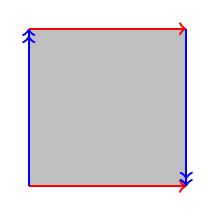
\begin{tikzpicture}
        \fill[color=black!25] (0,0) rectangle (2,2);
        \draw[thick,->, red] (0,0) -- ++(2,0);
        \draw[thick,->,red] (0,2) -- ++(2,0);
        \draw[thick,->>, blue] (0,0) -- ++(0,2);
        \draw[thick,->>,blue] (2,2) -- ++(0,-2);
    \end{tikzpicture}};

    \node (Tv) at (-3,-3) {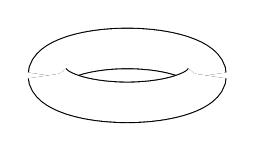
\begin{tikzpicture}[yscale=cos(70)]
        \draw[double distance=5mm] (0:1) arc (0:180:1);
        \draw[double distance=5mm] (180:1) arc (180:360:1);
      \end{tikzpicture}};
    \node (Kv) at (3,-3) {\begin{tikzpicture}[scale=0.25,use Hobby shortcut]
        \draw ([closed,blank=soft]0,0)
        \foreach \pt in {
        (-2,2),
        (2,2),
        (2,-2),
        (-2,-2),
        ([blank]-2,-1),
        (-1,-1),
        (1,-2),
        ([blank=soft]1,2),
        ([blank=soft]-1,1),
        (-3,3),
        (6,4.5),
        (4.5,-4.5),
        (-2.5,-6)
        } {
        .. ++\pt
        };
        % \draw[dashed,use previous hobby path={invert soft blanks}];
        \draw (0,0) .. +(-1,-1) .. ++(-2,-1);
        \draw[dashed] (0,0) .. +(-1,-.75) .. ++(-2,-1);
        \draw (-2.45,-3.9) .. +(3.3,-.75) .. (4.2,-3.95);
        \draw[dashed] (-2.45,-3.9) .. +(4.3,.5) .. (4.2,-3.95);
        \end{tikzpicture}};

        \draw[thick,->] (T) -- (Tv);
        \draw[thick,->] (K) -- (Kv);
    \end{tikzpicture}
    \caption{A torus and Klein bottle, with thanks to 
    \url{https://tex.stackexchange.com/q/77606/86}.}\label{fig:vanKampen}
\end{figure}

\index{topology}
Switch to topology.   Roll up a stretchy sheet of plastic along the following 
Van Kampen diagrams  viewed in Figure~\ref{fig:vanKampen} to make a torus $\mathbb{T}^2$ 
and a Klein bottle $\mathbb{K}$.  These are different, right?  Why?  Of course we use topology 
to prove the interesting bits.  In brief, the Seifert-van Kampen theorem applies: 
the loops $\pi_1(M^2)$ on a surfaces $M^2$ can each be decomposed into an 
equivalent sequence of blue loops $b$ and red loops $r$ as shown on Figure~\ref{fig:vanKampen}.
Loops that contract to nothing can therefore be understood as running forward
along blue and red loops in some order before reversing that whole process.  In particular
the loops along the boundary do just that.  
\begin{align*}
    \pi_1(\mathbb{T}^2) &= \text{ words over }\{b,r\} \text{ rewritten by }br=rb;
    \\
    \pi_1(\mathbb{K}^2) &= \text{ words over }\{b,r\} \text{ rewritten by } r=brb. 
\end{align*}
We use algebra to compute that those groups of loops are not the same so neither are the two spaces.

Other fields?  How many times in applied math, number theory, or combinatorics
do we end up solving something even if just a linear equation, or eigenvalue?
You don't have to be convinced but the evidence is there.

\index{algorithm}\index{Al Khwarizmi}\index{al Jabr}
Yet most of us do not want to be computers.  So what does an algebraist do 
when the questions come down to computing?  We put our energy into crafting 
algorithms to solve these problems.  In fact the word ``algorithm'' comes 
from al Khwarizmi whose influential book \emph{al Jabr} (the method of parts)
gave us the first detailed explanations of algebra.  Half of that book 
is a list of story problems solved by various algorithms in algebra.
\begin{quote}
    \textbf{The second method of algebra is to produce algorithms 
    that return solutions efficiently.}
\end{quote}

